\chapter{Simulation Data,Parameters and Testing Environment Evaluation Method}
\label{ch:data&model}

\section{Raw data for training}
Details of selected data is introduced in Chapter~\ref{ch:market}, the date range is from 2006-04-15 to 2016-04-15. As some data prior to the start date is hard to be collected. \\


Let $ EMA(n) $ represents $ n $ days EMA, similar to to $ SMA(n) $ , $ ROC(n) $ and $ RSI(n) $. $ MACD(m, n) $ means that the long term EMA of $ n $ days and short term EMA of $ m $ days, then the input features can be represented as [$ Price_{open}, Price_{high}, Price_{low}, Price_{close}, $ MACD(7, 14), MACD(12, 26), ROC(13), ROC(21), EMA(5), EMA(13), EMA(21), SMA(3), SMA(13), SMA(21), RSI(9), RSI(14), RSI(21), $ HIBOR_{\text{1 Year}} $, $ HIBOR_{\text{6 Months}} $, $ HIBOR_{\text{1 Week}} $, $ HIBOR_{\text{1 Month}} $, HKD/USD, HKD/EUR, HKD/CNY, HSI, SSE], feature number is 26 in total.\\


The stock chosen in this experiment is Cheung Kong (Holdings) Limited, CLP Holdings Limited, The Hong Kong and China Gas Company Limited, The Wharf (Holdings) Limited, HSBC Holdings plc, Power Assets Holdings Limited, Hoifu Energy Group Limited, PCCW Limited, Nine Express Limited and Hang Lung Group Limited. They are just the first 10 stocks in Yahoo Finance (0001.HK to 0010.HK).\\


Three of the above companies are top 50 in market capitalization (0001.HK, 0004.HK and 0002.HK). Two of them are top 20 active stocks in dollars (0001.HK and 0005.HK). One in finance (0005.HK), 3 in Utilities (0002.HK, 0003.HK and 0006.HK), two properties (0001.HK and 0004.HK).


\section{Detail Parameters of every training method}
Details of the parameters can be found in Table~\ref{tb:parameters}

\begin{table}[h]
	\centering
	\begin{tabular}{|l|l|l|}
		\hline
		\multicolumn{1}{|c|}{\textbf{Algorithm}} & \multicolumn{1}{c|}{\textbf{Parameters}} & \multicolumn{1}{c|}{\textbf{Optimize Method}} \\ \hline
		\textbf{\begin{tabular}[c]{@{}l@{}}Random Forest\\ (Classifier \& Regressor)\end{tabular}} & \begin{tabular}[c]{@{}l@{}}Trees Number: 40\\ Max Depth: 20\end{tabular} & NA \\ \hline
		\textbf{SVM} & \begin{tabular}[c]{@{}l@{}}Iterations: 100000\\ Learning rate: 0.001\end{tabular} & SGD \\ \hline
		\textbf{Logistic Regression} & \begin{tabular}[c]{@{}l@{}}Iterations: 100000\\ Learning rate: 0.001\end{tabular} & SGD \\ \hline
		\textbf{Linear Regression} & \begin{tabular}[c]{@{}l@{}}Iterations: 100000\\ Learning rate: 0.001\end{tabular} & SGD \\ \hline
		\textbf{ANN} & \begin{tabular}[c]{@{}l@{}}Iterations: 15\\ Learning rate: 0.0001\end{tabular} & BGD \\ \hline
	\end{tabular}
	\caption{Parameters of Every learning method}
	\label{tb:parameters}
\end{table}


The neural network is a four-layer (two hidden layer) model. A two-layer model is just same as linear regression. The reason for choosing 2 hidden layers is that "can represent an arbitrary decision boundary to arbitrary accuracy with rational activation functions and can approximate any smooth mapping to any accuracy"\cite{heaton2008introduction}.\\


To determine the number of neurons use in the hidden layers, Jeff Heaton also wrote in \cite{heaton2008introduction} that "The number of hidden neurons should be between the size of the input layer and the size of the output layer". So, in this study, the nodes number of the first hidden layer is $ \frac{2}{3} $ of that of the input layer, and that of the second is $ \frac{1}{3} $ of that of the input layer.\\


For the normalization method, the range of min-max normalizer is $ [-1, 1] $.


\section{Testing Environment}
The model of physical computer is Dell Inspiron Ins14VD-4516, details about the hardware information is showed in table~\ref{tb:hardwareConf}, software are listed in table~\ref{tb:softwareList}
\begin{table}[h]
	\centering
	\begin{tabular}{|l|l|}
		\hline
		\textbf{Name} & \textbf{Details} \\ \hline
		CPU & Intel Core i5 4200U \\ \hline
		Memory & DDR3L 1600MHz 8GB(4GBx2) \\ \hline
		Hard disk & 500GB 5400 rpm \\ \hline
	\end{tabular}
	\caption{Hardware information}
	\label{tb:hardwareConf}
\end{table}

\begin{table}[h]
	\centering
	\begin{tabular}{|l|l|}
		\hline
		\textbf{Name} & \textbf{Details} \\ \hline
		OS & Ubuntu (Host version: 16.04, Guest version: 14.04) \\ \hline
		Virtualbox & Version 5.0.20 r106931 \\ \hline
		Python & 2.7.6 \\ \hline
		Apache Spark & 1.6.1 \\ \hline
		Hadoop & 2.6.0 \\ \hline
	\end{tabular}r
	\caption{Primary Software information}
	\label{tb:softwareList}
\end{table}
\clearpage
The cluster is formed by three virtual machines (as figure~\ref{fg:clustur}). "Master" is NameNode for HDFS, and Master, HistoryServer for Spark. The other two virtual machines work as DataNode (for HDFS) and worker (for Spark). Every computer has 40GB hard disk, 2GB memory and 1 virtual CPU core.
\begin{figure}[h]
	\centering
	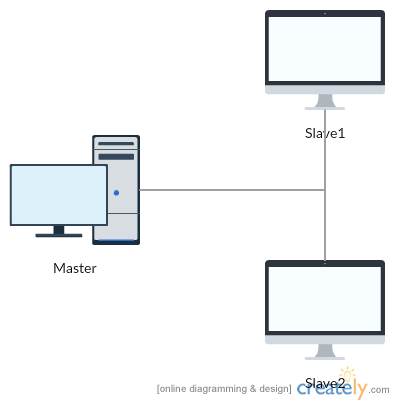
\includegraphics[width=0.6\textwidth]{ClusterStructure}
	\caption{Network Structure of the cluster}
	\label{fg:clustur}
\end{figure}
